\documentclass{article}
\usepackage{graphicx} % Required for inserting images
\usepackage{subcaption}
\usepackage{tikz}
\usepackage{tabularx}
\usepackage{pgfplots}
\usepackage{pgfplotstable}
\usepackage{amsmath,amssymb}
\usepackage{dblfloatfix}
\usepackage{placeins}
\usepgfplotslibrary{statistics,groupplots}
\pgfplotsset{compat=1.18}
\usepackage{comment}
\usepackage[top=1in,bottom=1in,left=1in,right=1in]{geometry} % Reduce the size of the margin


\usepackage{bm} % If you want bold math, but without the bloat of AMS packages
%\usepackage{vmargin} % To set page size

\usepackage{parskip}
%\usepackage{setspace}
%\doublespacing{}
%\usepackage{floatflt}
%\usepackage{program}
\usepackage{epsfig}
%\usepackage{subfigure}
%\usepackage{multitoc}
\usepackage{wrapfig}
%\usepackage[scriptsize]{caption}
\usepackage{amsmath, amsfonts, amsthm, amssymb}
\usepackage{algorithm}
\usepackage{algorithmic}
\usepackage{alltt}
\usepackage{url}
\usepackage{fancyvrb}
%\usepackage{helvet}
%\renewcommand{\familydefault}{\sfdefault}

% --- generated inputs (see README): every number and every plot below comes from results/
% Shared pgfplots setup and colormaps, rendered from templates/figure_preamble.tex.in
\pgfplotsset{table/search path={../results/figures}}
\input{../results/figures/figure_preamble.tex}%
% Where pgfplots looks for the figures' source tables
% The numbers quoted in the prose and captions, rendered by stages/stage7_figures.py
% GENERATED by stages/stage7_figures.py --prepare - do not edit.
% Every number the manuscript states in prose or a caption is defined here.
\newcommand{\valBinderFracPone}{1.000}
\newcommand{\valBinderFracPtwo}{0.982}
\newcommand{\valBinderFracPthree}{0.855}
\newcommand{\valBinderFracPfour}{0.855}
\newcommand{\valBinderFracPfive}{0.569}
\newcommand{\valBinderFracPsix}{0.734}
\newcommand{\valBinderFracPseven}{0.767}
\newcommand{\valBinderFracPeight}{0.887}
\newcommand{\valBinderFracPnine}{0.937}
\newcommand{\valBinderFracRfive}{0.569}
\newcommand{\valBinderFracnonRfive}{0.877}
\newcommand{\valMacroAucSCEPTR}{0.533}
\newcommand{\valMacroAucERGOtwo}{0.553}
\newcommand{\valMacroAucNetTCRtwotwo}{0.593}
\newcommand{\valMacroAucNetTCR}{0.609}
\newcommand{\valMacroAucTITAN}{0.614}
\newcommand{\valMacroAucPanPep}{0.619}
\newcommand{\valMacroAucEPACT}{0.629}
\newcommand{\valMacroAucERGO}{0.644}
\newcommand{\valNpairs}{3,591}
\newcommand{\valNpositive}{3,027}
\newcommand{\valNnegative}{564}
\newcommand{\valNmutations}{171}
\newcommand{\valNeligible}{113}
\newcommand{\valNexcluded}{58}
\newcommand{\valPosAucERGOPtwo}{0.731}
\newcommand{\valPosAucERGOPthree}{0.692}
\newcommand{\valPosAucERGOPfour}{0.726}
\newcommand{\valPosAucERGOPfive}{0.568}
\newcommand{\valPosAucERGOPsix}{0.594}
\newcommand{\valPosAucERGOPseven}{0.643}
\newcommand{\valPosAucERGOPeight}{0.664}
\newcommand{\valPosAucERGOPnine}{0.620}
\newcommand{\valPosAucEPACTPtwo}{0.762}
\newcommand{\valPosAucEPACTPthree}{0.688}
\newcommand{\valPosAucEPACTPfour}{0.623}
\newcommand{\valPosAucEPACTPfive}{0.514}
\newcommand{\valPosAucEPACTPsix}{0.561}
\newcommand{\valPosAucEPACTPseven}{0.626}
\newcommand{\valPosAucEPACTPeight}{0.764}
\newcommand{\valPosAucEPACTPnine}{0.653}
\newcommand{\valPosAucPanPepPtwo}{0.796}
\newcommand{\valPosAucPanPepPthree}{0.686}
\newcommand{\valPosAucPanPepPfour}{0.731}
\newcommand{\valPosAucPanPepPfive}{0.506}
\newcommand{\valPosAucPanPepPsix}{0.501}
\newcommand{\valPosAucPanPepPseven}{0.592}
\newcommand{\valPosAucPanPepPeight}{0.643}
\newcommand{\valPosAucPanPepPnine}{0.753}
\newcommand{\valPosAucTITANPtwo}{0.653}
\newcommand{\valPosAucTITANPthree}{0.609}
\newcommand{\valPosAucTITANPfour}{0.601}
\newcommand{\valPosAucTITANPfive}{0.588}
\newcommand{\valPosAucTITANPsix}{0.617}
\newcommand{\valPosAucTITANPseven}{0.602}
\newcommand{\valPosAucTITANPeight}{0.649}
\newcommand{\valPosAucTITANPnine}{0.646}
\newcommand{\valPosAucNetTCRPtwo}{0.673}
\newcommand{\valPosAucNetTCRPthree}{0.661}
\newcommand{\valPosAucNetTCRPfour}{0.614}
\newcommand{\valPosAucNetTCRPfive}{0.551}
\newcommand{\valPosAucNetTCRPsix}{0.536}
\newcommand{\valPosAucNetTCRPseven}{0.590}
\newcommand{\valPosAucNetTCRPeight}{0.635}
\newcommand{\valPosAucNetTCRPnine}{0.776}
\newcommand{\valPosAucNetTCRtwotwoPtwo}{0.693}
\newcommand{\valPosAucNetTCRtwotwoPthree}{0.544}
\newcommand{\valPosAucNetTCRtwotwoPfour}{0.511}
\newcommand{\valPosAucNetTCRtwotwoPfive}{0.489}
\newcommand{\valPosAucNetTCRtwotwoPsix}{0.641}
\newcommand{\valPosAucNetTCRtwotwoPseven}{0.577}
\newcommand{\valPosAucNetTCRtwotwoPeight}{0.772}
\newcommand{\valPosAucNetTCRtwotwoPnine}{0.621}
\newcommand{\valPosAucERGOtwoPtwo}{0.567}
\newcommand{\valPosAucERGOtwoPthree}{0.596}
\newcommand{\valPosAucERGOtwoPfour}{0.609}
\newcommand{\valPosAucERGOtwoPfive}{0.548}
\newcommand{\valPosAucERGOtwoPsix}{0.512}
\newcommand{\valPosAucERGOtwoPseven}{0.533}
\newcommand{\valPosAucERGOtwoPeight}{0.522}
\newcommand{\valPosAucERGOtwoPnine}{0.563}
\newcommand{\valPosAucSCEPTRPtwo}{0.501}
\newcommand{\valPosAucSCEPTRPthree}{0.578}
\newcommand{\valPosAucSCEPTRPfour}{0.521}
\newcommand{\valPosAucSCEPTRPfive}{0.519}
\newcommand{\valPosAucSCEPTRPsix}{0.512}
\newcommand{\valPosAucSCEPTRPseven}{0.552}
\newcommand{\valPosAucSCEPTRPeight}{0.499}
\newcommand{\valPosAucSCEPTRPnine}{0.603}
\newcommand{\valBestModelPtwo}{PanPep}
\newcommand{\valBestModelPthree}{ERGO}
\newcommand{\valBestModelPfour}{PanPep}
\newcommand{\valBestModelPfive}{TITAN}
\newcommand{\valBestModelPsix}{NetTCR2.2}
\newcommand{\valBestModelPseven}{ERGO}
\newcommand{\valBestModelPeight}{NetTCR2.2}
\newcommand{\valBestModelPnine}{NetTCR}
\newcommand{\valRfiveAucERGO}{0.568}
\newcommand{\valNonRfiveAucERGO}{0.660}
\newcommand{\valRfiveAucEPACT}{0.514}
\newcommand{\valNonRfiveAucEPACT}{0.652}
\newcommand{\valRfiveAucPanPep}{0.506}
\newcommand{\valNonRfiveAucPanPep}{0.642}
\newcommand{\valRfiveAucTITAN}{0.588}
\newcommand{\valNonRfiveAucTITAN}{0.619}
\newcommand{\valRfiveAucNetTCR}{0.551}
\newcommand{\valNonRfiveAucNetTCR}{0.620}
\newcommand{\valRfiveAucNetTCRtwotwo}{0.489}
\newcommand{\valNonRfiveAucNetTCRtwotwo}{0.614}
\newcommand{\valRfiveAucERGOtwo}{0.548}
\newcommand{\valNonRfiveAucERGOtwo}{0.554}
\newcommand{\valRfiveAucSCEPTR}{0.519}
\newcommand{\valNonRfiveAucSCEPTR}{0.536}
\newcommand{\valNrfive}{19}
\newcommand{\valNnonrfive}{94}
\newcommand{\valBestModelRfive}{TITAN}
\newcommand{\valRhoDisruption}{0.723}
\newcommand{\valPDisruption}{1.6\times10^{-19}}
\newcommand{\valRhoBinderLoss}{0.876}
\newcommand{\valPBinderLoss}{6.7\times10^{-37}}
\newcommand{\valNmodels}{8}
\newcommand{\valNtcrs}{21}
\newcommand{\valNpeptides}{172}
\newcommand{\valOverlapModel}{NetTCR-2.2}
\newcommand{\valOverlapPeptidesWord}{one}
\newcommand{\valOverlapPairRowsWord}{two}
\newcommand{\valOvlPepUniqERGO}{0}
\newcommand{\valOvlPepPctERGO}{0.0}
\newcommand{\valOvlPepRowsERGO}{0}
\newcommand{\valOvlPepRowPctERGO}{0.0}
\newcommand{\valOvlPairRowsERGO}{0}
\newcommand{\valOvlPairPctERGO}{0.0}
\newcommand{\valOvlPepUniqERGOtwo}{0}
\newcommand{\valOvlPepPctERGOtwo}{0.0}
\newcommand{\valOvlPepRowsERGOtwo}{0}
\newcommand{\valOvlPepRowPctERGOtwo}{0.0}
\newcommand{\valOvlPairRowsERGOtwo}{0}
\newcommand{\valOvlPairPctERGOtwo}{0.0}
\newcommand{\valOvlPepUniqNetTCR}{0}
\newcommand{\valOvlPepPctNetTCR}{0.0}
\newcommand{\valOvlPepRowsNetTCR}{0}
\newcommand{\valOvlPepRowPctNetTCR}{0.0}
\newcommand{\valOvlPairRowsNetTCR}{0}
\newcommand{\valOvlPairPctNetTCR}{0.0}
\newcommand{\valOvlPepUniqNetTCRtwotwo}{1}
\newcommand{\valOvlPepPctNetTCRtwotwo}{0.6}
\newcommand{\valOvlPepRowsNetTCRtwotwo}{21}
\newcommand{\valOvlPepRowPctNetTCRtwotwo}{0.6}
\newcommand{\valOvlPairRowsNetTCRtwotwo}{2}
\newcommand{\valOvlPairPctNetTCRtwotwo}{0.1}
\newcommand{\valOvlPepUniqTITAN}{0}
\newcommand{\valOvlPepPctTITAN}{0.0}
\newcommand{\valOvlPepRowsTITAN}{0}
\newcommand{\valOvlPepRowPctTITAN}{0.0}
\newcommand{\valOvlPairRowsTITAN}{0}
\newcommand{\valOvlPairPctTITAN}{0.0}
\newcommand{\valOvlPepUniqEPACT}{0}
\newcommand{\valOvlPepPctEPACT}{0.0}
\newcommand{\valOvlPepRowsEPACT}{0}
\newcommand{\valOvlPepRowPctEPACT}{0.0}
\newcommand{\valOvlPairRowsEPACT}{0}
\newcommand{\valOvlPairPctEPACT}{0.0}
\newcommand{\valOvlPepUniqPanPep}{0}
\newcommand{\valOvlPepPctPanPep}{0.0}
\newcommand{\valOvlPepRowsPanPep}{0}
\newcommand{\valOvlPepRowPctPanPep}{0.0}
\newcommand{\valOvlPairRowsPanPep}{0}
\newcommand{\valOvlPairPctPanPep}{0.0}
\newcommand{\valOvlPepUniqSCEPTR}{0}
\newcommand{\valOvlPepPctSCEPTR}{0.0}
\newcommand{\valOvlPepRowsSCEPTR}{0}
\newcommand{\valOvlPepRowPctSCEPTR}{0.0}
\newcommand{\valOvlPairRowsSCEPTR}{0}
\newcommand{\valOvlPairPctSCEPTR}{0.0}
%
\title{Benchmarking TCR–Epitope Recognition Models across Antigen Mutations}
\author{Yiming Liao, Yiheng Li, Ning Jiang, Bo Li, Keke Chen}
\begin{comment}
\email{lib3@chop.edu}
\author*[1]{Keke Chen} \email{kekechen@umbc.edu}
\affil[1]{Trustworthy and Intelligent Computing Lab (TAIC), Department of Computer Science and Electrical Engineering, University of Maryland, Baltimore County, Maryland, 21250}
\affil[2]{Children's Hospital of Philadelphia, Philadelphia, PA, 19104}
\affil[3]{Department of Bioengineering, University of Pennsylvania, Philadelphia, PA, 19104}
\end{comment}
\date{}


\begin{document}
\maketitle

\begin{abstract}

\textbf{Motivation:}
T cell receptor (TCR)--epitope prediction models are commonly evaluated on collections of positive and negative TCR--peptide pairs or on generalization to unseen epitopes. These settings do not directly test whether models can reproduce experimentally observed changes in TCR recognition caused by controlled antigen sequence perturbations.

\textbf{Results:}
We introduce a mutation-aware evaluation framework in which all test peptides are single-amino-acid variants of a common reference antigen and prediction performance is assessed against experimentally measured retention or loss of TCR recognition. Using the HLA-A*02:01-restricted SARS-CoV-2 epitope YLQPRTFLL, we constructed a benchmark containing all \valNmutations\ possible single-amino-acid substitutions evaluated across \valNtcrs\ TCRs, yielding \valNpairs\ TCR--mutant interactions. Eight representative prediction models were assessed using mutation-specific standardized partial ROC-AUC at FPR $\leq 0.1$. Overall performance was modest, with the best Macro AUC$_{0.1}$ below 0.65, and prediction quality varied substantially across individual mutations and peptide positions. No model performed best throughout the antigen sequence. Mutations at the experimentally restrictive R5 position were consistently more difficult to predict than mutations at other positions. More generally, cross-model prediction performance declined as mutations produced stronger or broader experimental losses of TCR recognition, with Spearman correlations of $\rho=-\valRhoDisruption$ for recognition disruption and $\rho=-\valRhoBinderLoss$ for binder-loss fraction. These results reveal a systematic failure mode not captured by conventional pairwise benchmarks: current models are least reliable for antigen mutations with the largest experimentally observed effects on TCR recognition.

\textbf{Availability and Implementation:}
Code and processed benchmark data will be made publicly available upon publication.

\end{abstract}
\section{Introduction}

T cell receptors (TCRs) recognize antigenic peptides presented by major
histocompatibility complex (MHC) molecules and thereby mediate
antigen-specific cellular immune responses
\cite{garcia05}. Characterizing TCR--peptide--MHC (pMHC) recognition is
important for understanding immune responses to infection, vaccination,
cancer, and autoimmunity, as well as for the development of T-cell-based
diagnostics and therapeutics. Experimental methods such as pMHC multimer
staining provide direct measurements of antigen-specific T cells
\cite{dolton14}, while more recent high-throughput approaches enable
multiplexed mapping of TCR specificity across large antigen panels
\cite{wenzhangFrameworkHighlyMultiplexed2021,joglekar2021t}.
Nevertheless, exhaustive experimental characterization remains difficult
because of the enormous combinatorial space of TCR and antigen sequences.

Computational TCR--epitope prediction has therefore emerged as an important
complement to experimental characterization. Over the past decade, a broad
range of sequence-based and machine-learning approaches have been developed
to predict TCR antigen specificity, using representations ranging from
CDR3-based inputs to paired TCR $\alpha\beta$ chains, additional CDR loops,
gene usage, and HLA context. Recent community benchmarking efforts such as
IMMREP22 and IMMREP23 have evaluated many of these approaches under common
test settings and highlighted both progress and substantial remaining
limitations in TCR--epitope prediction
\cite{nielsen24,meysman23}.

Despite continued methodological development, reliable generalization
remains a major challenge. Previous studies have shown that TCR-binding
predictors can exhibit substantial performance degradation when evaluated on
previously unseen peptides
\cite{grazioli2022tcr}. The IMMREP23 community benchmark similarly
demonstrated the difficulty of generalizing to new epitopes
\cite{nielsen24}. Independent comparisons of TCR--pMHC prediction
methods have further shown that performance can depend strongly on training
data and evaluation-set composition
\cite{lu2026assessment}.
Together, these studies demonstrate that strong performance on conventional
TCR--epitope benchmarks does not necessarily imply robust generalization to
new antigen-recognition settings.

Most existing evaluations nevertheless formulate TCR specificity primarily
as a pairwise discrimination problem: given a TCR and an epitope, the model
is evaluated on whether it distinguishes experimentally positive from
negative interactions. This formulation does not directly address an
important biological use case. Antigen sequences vary and evolve, and even
a single amino-acid substitution can substantially alter TCR recognition.
Because TCRs must recognize related but non-identical peptide sequences,
cross-reactivity is an intrinsic property of cellular immunity
\cite{sewell12}. At the same time, antigen substitutions can alter or
eliminate recognition by particular T-cell populations. Such effects have
been observed for SARS-CoV-2 variants, where mutations can differentially
affect CD8$^+$ T-cell responses
\cite{buckley2023systems}, and cross-reactive T-cell recognition has been an
important consideration in understanding immunity to SARS-CoV-2
\cite{yang2023sars}.

Importantly, the effects of antigen mutations are structured rather than
uniform. Some peptide positions tolerate broad amino-acid variation, whereas
others are strongly constrained, and mutations at the same position can
affect different TCRs differently. This raises a complementary
model-evaluation question that is not captured by conventional pairwise
benchmarks:
\emph{can current TCR--epitope prediction models reproduce experimentally
observed changes in TCR recognition caused by antigen mutations?}
Answering this question requires an evaluation design in which mutations are
systematically related to a common reference antigen and both retained and
lost recognition are measured experimentally.

The TCR Fingerprinting study of Malone et
al.~\cite{malone2025fingerprinting} provides such an opportunity. The study
systematically characterized recognition of the HLA-A*02:01-restricted
SARS-CoV-2 epitope YLQPRTFLL (YLQ) and its single-amino-acid variants. The
experimental panel contains the reference peptide together with all 171
possible single-amino-acid substitutions across its nine positions.
Twenty-one TCRs were evaluated against this peptide panel using
background-normalized pMHC staining, producing quantitative recognition
measurements and experimentally defined binding outcomes. The resulting data
reveal a highly structured mutation landscape in which some positions are
broadly tolerant, others produce greater recognition losses, and the central
R5 residue is particularly restrictive
\cite{malone2025fingerprinting}.

These data differ fundamentally from benchmark collections assembled from
unrelated TCR--epitope pairs. Because every mutant peptide represents a
controlled perturbation of the same reference antigen, the dataset enables
prediction performance to be evaluated at the level of individual mutations
and antigen positions. Moreover, non-binding interactions are experimentally
observed rather than generated through random reassignment of TCRs and
peptides. This provides an opportunity to examine not only whether models
distinguish binding from non-binding interactions, but also where in the
mutation landscape current models succeed or fail.

In this study, we construct a mutation-aware computational benchmark from
the Fingerprinting measurements and use it to evaluate eight representative
TCR--epitope prediction models. The evaluated methods span different model
architectures, TCR input representations, and training-data sources. We use
a model-independent evaluation procedure in which prediction performance is
computed separately for individual antigen mutations and then summarized
across mutations and peptide positions. Because the evaluated models were
trained using different public resources, we additionally examine
model-specific training--benchmark overlap before evaluation. We have found that overlap with
the Fingerprinting panel does not exist for most models and is very limited for
one model.

Our evaluation reveals several consistent limitations of current prediction
methods. Overall mutation-level discrimination is modest, with the best
model achieving a Macro AUC$_{0.1}$ below 0.65. Prediction performance also
varies substantially across individual mutations and peptide positions, and
no single model performs best throughout the antigen sequence. In
particular, substitutions at the experimentally restrictive R5 position are
more difficult to predict than mutations at the remaining positions. More
broadly, prediction performance decreases systematically as mutations
produce stronger or more widespread experimental losses of TCR recognition.
Thus, the mutations with the largest experimentally observed effects are
also among the most challenging for current computational models.


The main contributions of this study are threefold:
\begin{itemize}
    \item We construct a mutation-aware computational benchmark from
    systematic experimental perturbations of a common reference antigen.
    Because all test peptides differ from the same epitope by a single
    amino-acid substitution, the benchmark enables controlled evaluation of
    TCR--epitope recognition across a densely sampled local mutation
    landscape of 171 antigen variants.

    \item We introduce a mutation-resolved evaluation framework that exposes where current predictors succeed or fail within a controlled antigen landscape, including mutation-specific, position-specific, and R5-specific behavior that is hidden by aggregate TCR–epitope classification metrics.

    \item Through systematic evaluation of eight representative prediction
    models, we identify a consistent failure mode of current methods:
    prediction performance is strongly mutation dependent and deteriorates
    for antigen substitutions that produce larger or broader experimentally
    observed losses of TCR recognition.
\end{itemize}
Together, these results extend evaluation of TCR specificity prediction
beyond the conventional question of whether a TCR recognizes an antigen
toward the more demanding question of whether computational models can
predict how antigen sequence variation changes TCR recognition.


\section{Materials and Methods}

\subsection{Overview of the Mutation-Aware Benchmarking Framework}

This study does not propose a new T cell receptor (TCR)--epitope prediction
model. Instead, we develop a model-independent benchmarking framework to
evaluate whether existing computational models reproduce experimentally
observed effects of antigen mutations on TCR recognition. The overall workflow
is illustrated in Fig.~\ref{fig:framework}.

\begin{figure}[t]
    \centering
    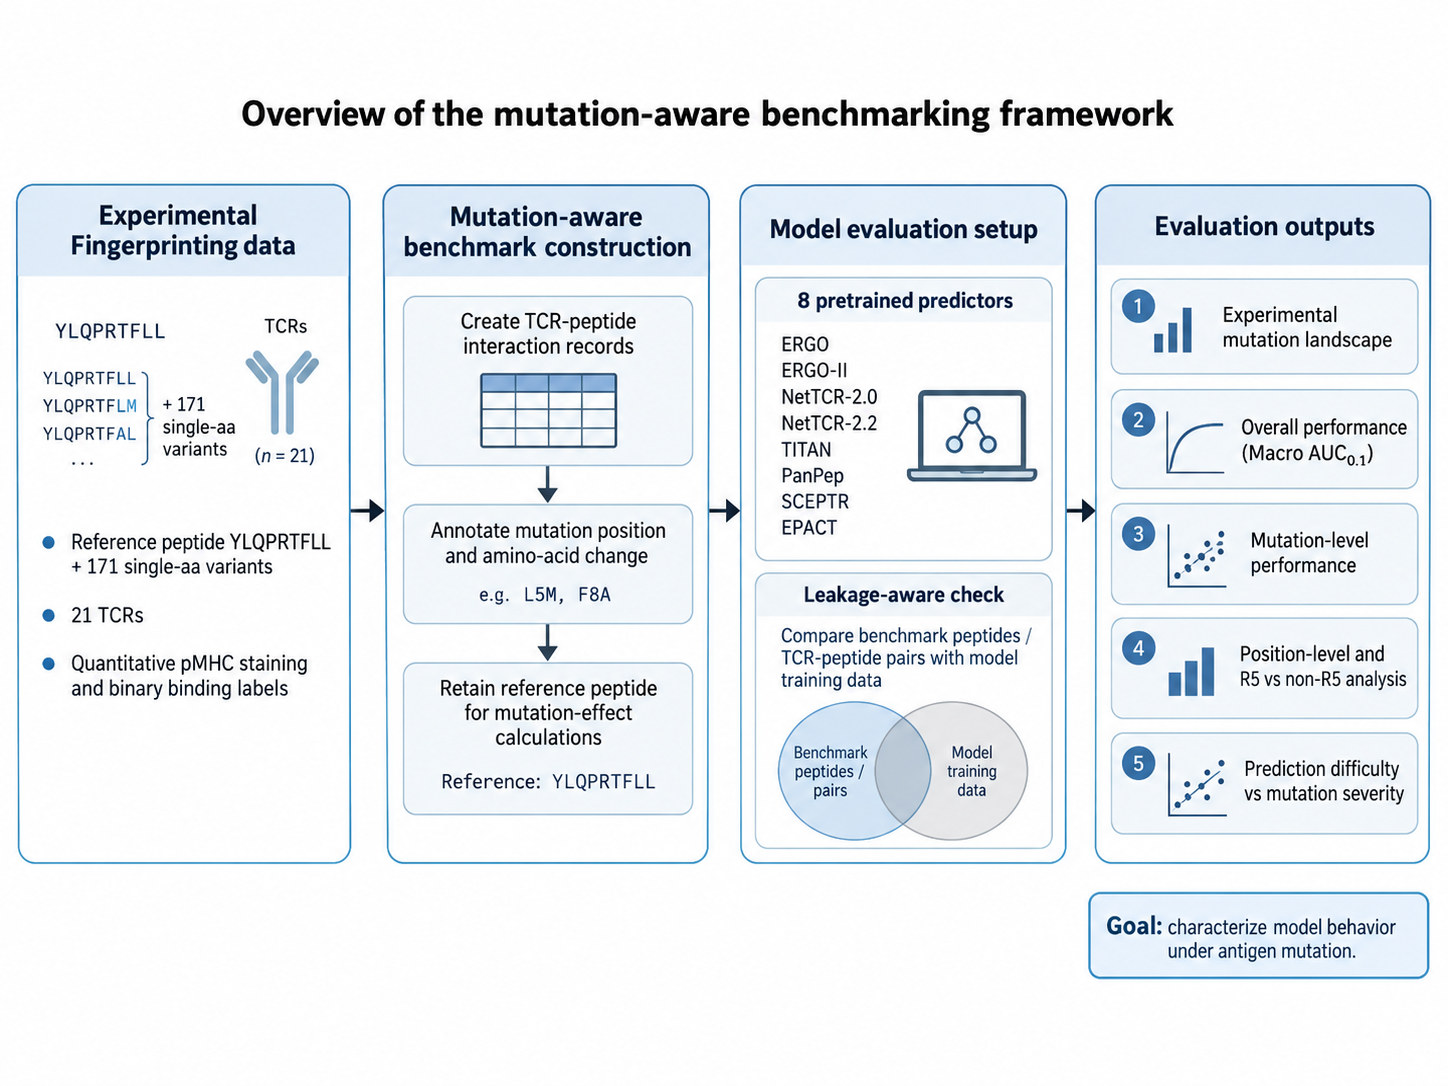
\includegraphics[width=0.9\linewidth]{figures/framework.png}
    \caption{
    Overview of the mutation-aware benchmarking framework. The workflow
    starts from the experimental Fingerprinting dataset and model training
    data, performs overlap screening and model inference, and then evaluates
    prediction performance at the mutation, position, and mutation-severity
    levels.
    }
    \label{fig:framework}
\end{figure}
The framework consists of five major components:
(1) construction of a computational benchmark from systematic
single-amino-acid mutagenesis experiments;
(2) examination of the training data used by individual prediction models to
identify potential training--benchmark overlap;
(3) inference of TCR--epitope prediction scores using the original pretrained
models;
(4) mutation- and position-level evaluation using experimentally measured
binding outcomes; and
(5) analysis of whether model performance deteriorates systematically for
mutations that produce stronger experimentally observed disruption of TCR
recognition.

Rather than treating all TCR--peptide interactions as independent test
examples, the evaluation preserves the structured relationship among peptide
variants derived from the same reference antigen. This design enables model
performance to be examined at the level of individual antigen mutations,
peptide positions, and biologically consequential mutation classes.


\subsection{Experimental Fingerprinting Dataset}

\subsubsection{TCRs and antigen mutation panel}

The experimental data used in this study were generated using the TCR
fingerprinting approach reported by Malone et
al.~\cite{malone2025fingerprinting}. The study characterized recognition of
the immunodominant SARS-CoV-2 epitope YLQPRTFLL (YLQ), presented by
HLA-A*02:01, together with a systematic panel of single-amino-acid
substitutions.

The complete panel contains \valNpeptides\ peptide species: the reference YLQPRTFLL
peptide and \valNmutations\ single-amino-acid variants corresponding to all 19 possible
non-reference amino acids at each of the nine peptide positions. These
peptides were evaluated against \valNtcrs\ TCRs. Twenty TCRs were identified using
the reference YLQ peptide, whereas one additional TCR was identified using a
pool of R5-mutant peptides.

The systematic mutation design differs from conventional TCR--epitope
datasets assembled from unrelated positive and negative interactions. Each
mutant differs from the reference antigen at exactly one defined residue,
allowing the effect of antigen sequence perturbation on TCR recognition to be
examined in a controlled mutation landscape.


\subsubsection{Experimental pMHC-recognition measurements}

TCR-specific peptide--MHC (pMHC) recognition was measured by staining
TCR-transduced J76 cells with individual pMHC tetramers. Background staining
was measured using TCR-negative J76 cells. For TCR $i$ and peptide $j$, the
quantitative experimental recognition signal was represented as

\begin{equation}
B_{ij}
=
\log_2
\left(
\frac{\mathrm{MFI}_{\mathrm{TCR}^{+},ij}}
     {\mathrm{MFI}_{\mathrm{TCR}^{-},j}}
\right),
\label{eq:binding_signal}
\end{equation}

where $\mathrm{MFI}_{\mathrm{TCR}^{+},ij}$ denotes the pMHC staining
intensity measured for TCR-transduced cells and
$\mathrm{MFI}_{\mathrm{TCR}^{-},j}$ denotes the corresponding background
staining intensity measured using TCR-negative cells for peptide $j$.

Following the experimental definition used in the original study,
TCR--pMHC interactions were classified as binders when

\begin{equation}
y_{ij}
=
\begin{cases}
1, & B_{ij} > 1,\\
0, & B_{ij} \leq 1.
\end{cases}
\label{eq:binary_label}
\end{equation}

Thus, the Fingerprinting dataset provides two complementary experimental
endpoints: a continuous background-normalized pMHC-recognition measurement
and a binary indicator of experimentally retained binding.

The original study also evaluated the HLA-A*02:01 binding capacity of the
mutant peptides. Peptides were assessed using NetMHCpan 4.1, with predicted
strong and weak MHC binders defined by \%Rank $<0.5$ and \%Rank $<2$,
respectively. Peptide--MHC stability was additionally evaluated
experimentally using a T2 stabilization assay. These controls reduce the
possibility that apparent changes in TCR recognition are driven primarily by
failure of peptide presentation rather than altered TCR recognition.


\subsection{Construction of the Fingerprinting Computational Benchmark}

The Fingerprinting measurements were converted into a structured
mutation-aware computational benchmark. Each benchmark record corresponds to
a specific TCR and peptide species and contains the TCR sequence information,
peptide sequence, mutation position, reference and substituted amino acids,
quantitative experimental recognition measurement, and binary experimental
binding label.

For mutant peptide $j$ and TCR $i$, a benchmark interaction can be
represented as

\begin{equation}
D_{ij}
=
\left(
T_i,
P_j,
k_j,
a_j^{\mathrm{ref}},
a_j^{\mathrm{mut}},
B_{ij},
y_{ij}
\right),
\label{eq:benchmark_record}
\end{equation}

where $T_i$ denotes the TCR sequence information, $P_j$ denotes the mutant
peptide sequence, $k_j$ is the mutation position,
$a_j^{\mathrm{ref}}$ and $a_j^{\mathrm{mut}}$ are the reference and
substituted amino acids, respectively, and $B_{ij}$ and $y_{ij}$ are the
continuous and binary experimental measurements.

The unmutated YLQPRTFLL peptide was retained as the experimental reference
for mutation-effect calculations but was excluded from mutation-level
prediction evaluation. The resulting mutation benchmark therefore contains
\valNmutations\ distinct single-amino-acid substitutions and \valNpairs\ TCR--mutant
interactions.


\subsection{Evaluated TCR--Epitope Prediction Models}

We evaluated eight existing TCR--epitope prediction models:
ERGO~\cite{idospringerPredictionSpecificTCRPeptide2020},
ERGO-II~\cite{springer2021contribution},
NetTCR-2.0~\cite{montemurro2021nettcr},
NetTCR-2.2~\cite{mathiasfynbojensenEnhancingTCRSpecificity2024},
TITAN~\cite{annaweberTITANTcellReceptor2021},
PanPep~\cite{gao2023pan},
SCEPTR~\cite{nagano2024contrastive},
and EPACT~\cite{zhang2024epitope}.

These models were selected to provide a diverse cross-section of recent
TCR-specificity predictors that are publicly available and can be applied
to the Fingerprinting dataset without retraining. Collectively, they span
different generations of model development, TCR input representations,
training-data sources, and modeling strategies, ranging from relatively
compact CDR3-based predictors to models that incorporate paired
$\alpha\beta$ chains, additional CDR loops, gene usage, and HLA context.
The purpose of this selection is not to establish an exhaustive ranking of
all published TCR--epitope predictors, but to assess whether current
representative methods with substantially different designs exhibit similar
strengths and limitations when evaluated on a controlled antigen-mutation
benchmark.
The Fingerprinting dataset provides a superset of the sequence and annotation
information required by these models, including paired TCR $\alpha/\beta$
sequences, CDR information, V/J gene annotations, peptide sequence, and the
HLA-A*02:01 restriction. For each predictor, we therefore extracted the
subset of benchmark fields required by its published input representation.
This allows all models to be evaluated on the same underlying experimental
interactions while preserving their original input specifications.

The evaluated models differ substantially in the amount of TCR and pMHC
information incorporated during prediction. ERGO uses CDR3$\beta$ and peptide
sequence, whereas ERGO-II can additionally incorporate paired
CDR3$\alpha$, V/J gene usage, MHC allele, and T-cell type. NetTCR-2.0 uses
CDR3$\alpha$ and/or CDR3$\beta$ together with peptide sequence, while
NetTCR-2.2 incorporates all six CDR1--3 loops from the paired
$\alpha$ and $\beta$ chains. TITAN and PanPep primarily use TCR$\beta$
sequence information together with the peptide sequence. In contrast,
SCEPTR and EPACT use richer paired $\alpha\beta$ TCR representations and
jointly model the peptide together with HLA information.

The models were originally developed using different combinations of public
and experimentally generated TCR--epitope datasets, including McPAS-TCR,
VDJdb, IEDB, PIRD, TBAdb, 10x Genomics multimer data, and other curated
cohorts. These differences in training data motivate the model-specific
training--benchmark overlap analysis described in the following subsection.

For each model, we used the publicly released pretrained implementation and
followed the corresponding inference procedure. All evaluated models produced
a continuous binding score in the range $[0,1]$, with larger values indicating
stronger predicted TCR--epitope binding. Because the internal transformation
used to obtain these scores is model-specific, we treated the released model
score as the prediction output without additional calibration or rescaling.
The continuous scores were used directly for ROC-based evaluation and were
not converted to binary predictions using model-specific thresholds.

Table~\ref{tab:models} summarizes the input fields, training data, output
representation, and implementation information for the eight evaluated
models.

\begin{table*}[h]
\scriptsize
\centering
\begin{tabularx}{\textwidth}{l X X X X l}
\hline
\textbf{Model} &
\textbf{TCR input used} &
\textbf{Peptide input} &
\textbf{MHC input} &
\textbf{Training data} &
\textbf{Version} \\
\hline

ERGO &
CDR3$\beta$ &
Epitope sequence &
Not used &
McPAS-TCR and VDJdb; additional tumor-derived data &
\\

ERGO-II &
CDR3$\beta$ with optional CDR3$\alpha$; V/J gene usage and T-cell type can also be incorporated &
Epitope sequence &
MHC allele can be included &
McPAS-TCR and VDJdb; 10x data excluded during training-data construction &
\\

NetTCR-2.0 &
CDR3$\alpha$ and/or CDR3$\beta$, with paired chains used when available &
Epitope sequence &
Not explicitly modeled &
IEDB and VDJdb positive interactions; 10x data used for negative examples &
\\

NetTCR-2.2 &
CDR1--3 loops from both TCR$\alpha$ and TCR$\beta$ chains &
Epitope sequence &
Not explicitly modeled &
Curated IEDB and VDJdb binders; denoised 10x data used for negative examples &
\\

TITAN &
CDR3$\beta$ or TCR$\beta$ sequence representation &
Epitope sequence or molecular representation &
Not used &
Curated TCR--epitope interactions compiled primarily from McPAS-TCR and VDJdb-related sources &
\\

PanPep &
CDR3$\beta$ &
Epitope sequence &
Not explicitly modeled &
IEDB, VDJdb, PIRD, McPAS-TCR, and additional SARS-CoV-2 cohort data &
\\

SCEPTR &
Paired TCR$\alpha\beta$ using all six CDR loops &
Epitope sequence &
HLA jointly modeled with peptide &
Pretraining on approximately 842,000 paired $\alpha\beta$ clonotypes; downstream TCR--pMHC training/evaluation using curated antigen-specific data &
\\

EPACT &
Paired TCR$\alpha\beta$ &
Epitope sequence &
HLA class I jointly modeled &
IEDB, VDJdb, McPAS-TCR, TBAdb, SARS-CoV-2 datasets, and 10x multimer data &
\\

\hline
\end{tabularx}

\caption{
TCR--epitope prediction models evaluated in this study. The
Fingerprinting dataset provides the sequence and annotation information
required by all models, and each predictor was supplied with the subset of
fields corresponding to its published input representation. All models
produced continuous binding scores in the range $[0,1]$, which were used
directly for ROC-based evaluation without additional calibration or
model-specific thresholding. The exact software or checkpoint version used
for each model will be added after implementation verification.
}
\label{tab:models}
\end{table*}

\subsection{Model-Specific Training--Benchmark Overlap Control}

Potential training--benchmark overlap was examined separately for each model
because the evaluated predictors were developed using different combinations
of public TCR databases and experimental datasets. Original training datasets
released by the model developers were used whenever available. When exact
training sets were not publicly released, they were reconstructed from the
data sources and preprocessing procedures described in the corresponding
publications.

We distinguished several forms of prior exposure that may affect benchmark
interpretation, including overlap at the peptide level and overlap involving
specific TCR--peptide combinations. Peptide overlap was defined as the
presence of an identical benchmark peptide sequence in the model's training
data. We additionally examined exact CDR3$\beta$--peptide matches to identify
benchmark interactions that may have been directly represented during model
development.

Overall, training--benchmark overlap was minimal. For ERGO, ERGO-II,
NetTCR-2.0, TITAN, EPACT, PanPep, and SCEPTR, none of the \valNpeptides\ Fingerprinting
peptides were identified in the corresponding training data, and no exact
CDR3$\beta$--peptide matches were observed. \valOverlapModel\ showed only limited
overlap: \valOverlapPeptidesWord\ of the \valNpeptides\ peptide species (\valOvlPepPctNetTCRtwotwo\%) was present in its training
data, corresponding to \valOvlPepRowsNetTCRtwotwo\ benchmark rows (\valOvlPepRowPctNetTCRtwotwo\% of interactions), and only
\valOverlapPairRowsWord\ benchmark rows (\valOvlPairPctNetTCRtwotwo\%) matched an exact CDR3$\beta$--peptide combination.

These results indicate that the Fingerprinting benchmark is largely
independent of the training data used by the evaluated models. The extremely
limited overlap observed for NetTCR-2.2 was recorded explicitly and taken
into account during leakage-aware evaluation.

Importantly, prior exposure to the reference YLQ sequence was distinguished
from direct exposure to individual mutant interactions. Because the benchmark
is designed to evaluate the effects of antigen perturbation around a common
reference sequence, knowledge of the reference antigen does not necessarily
constitute the same form of leakage as direct exposure to a benchmark mutant
or an identical TCR--mutant pair.

\begin{table}[t]
\small
\centering
\caption{
Training--benchmark overlap between the Fingerprinting dataset and the
training data used by the evaluated prediction models.
}
\label{tab:leakage}
% Table 2: generated by stages/stage6_tables.py from its own source table
% GENERATED by stages/stage6_tables.py from table2_overlap_source.csv - do not edit.
% Training--benchmark overlap between the Fingerprinting dataset and the training data used by the evaluated prediction models.
\begin{tabular}{lccc}
\hline
Model & Peptide overlap & Rows with peptide overlap & Exact CDR3$\beta$--peptide rows \\
\hline
ERGO & 0/172 (0.0\%) & 0 (0.0\%) & 0 (0.0\%) \\
ERGO-II & 0/172 (0.0\%) & 0 (0.0\%) & 0 (0.0\%) \\
NetTCR-2.0 & 0/172 (0.0\%) & 0 (0.0\%) & 0 (0.0\%) \\
NetTCR-2.2 & 1/172 (0.6\%) & 21 (0.6\%) & 2 (0.1\%) \\
TITAN & 0/172 (0.0\%) & 0 (0.0\%) & 0 (0.0\%) \\
EPACT & 0/172 (0.0\%) & 0 (0.0\%) & 0 (0.0\%) \\
PanPep & 0/172 (0.0\%) & 0 (0.0\%) & 0 (0.0\%) \\
SCEPTR & 0/172 (0.0\%) & 0 (0.0\%) & 0 (0.0\%) \\
\hline
\end{tabular}%
%
\end{table}

\subsection{Experimental Characterization of the Mutation Landscape}

Before evaluating computational predictions, we summarized the experimentally
observed mutation landscape to establish the biological reference against
which model performance was interpreted. 

For each mutation $j$, the experimentally observed binder-retention fraction
was calculated as

\begin{equation}
R_j
=
\frac{1}{N_j}
\sum_{i=1}^{N_j} y_{ij},
\label{eq:binder_fraction}
\end{equation}

where $N_j$ is the number of TCRs evaluated against mutation $j$ and
$y_{ij}$ is the experimentally defined binary binding label.

Position-level experimental tolerance was then quantified by averaging
$R_j$ over the 19 possible substitutions occurring at each peptide
position. At position P1, all 19 single-amino-acid substitutions retained experimentally defined
binding across the tested TCRs, corresponding to a position-level mean
binder-retention fraction of 1.0. P1 therefore represents a highly
mutation-tolerant position in the experimental recognition landscape. 
This analysis was used to identify relatively mutation-tolerant
and mutation-restrictive regions of the YLQPRTFLL epitope.

Because substitutions at the central R5 residue exhibited particularly
strong recognition losses in the experimental data, binder-retention
fractions for R5 substitutions were additionally compared with those for
mutations at all remaining peptide positions (excluding P1).


\subsection{Model Inference and Mutation-Level Prediction Evaluation}

For model $m$, let $S_{ij}^{(m)}$ denote the continuous prediction score
assigned to TCR $i$ and mutant peptide $j$. Prediction performance was
evaluated using the standardized partial area under the receiver operating
characteristic curve over the low-false-positive-rate region
$\mathrm{FPR}\leq0.1$, denoted AUC$_{0.1}$.

AUC$_{0.1}$ was calculated using the continuous model prediction scores and
the experimentally defined binary labels. The standardized partial-AUC
formulation was used such that a random classifier has an expected value of
0.5 and perfect discrimination has a value of 1.0. In implementation, this
corresponds to the standardized partial ROC-AUC computed with
\texttt{roc\_auc\_score(..., max\_fpr=0.1)} in scikit-learn.

The fundamental evaluation unit was an individual antigen mutation. For each
mutation $j$, AUC$_{0.1}$ was calculated across the TCRs evaluated against
that mutant peptide:

\begin{equation}
A_j^{(m)}
=
\mathrm{AUC}_{0.1}
\left(
\{y_{ij}\}_{i=1}^{N_j},
\{S_{ij}^{(m)}\}_{i=1}^{N_j}
\right).
\label{eq:mutation_auc}
\end{equation}

ROC-based evaluation requires both experimentally positive and negative
interactions. Mutations for which all tested TCRs belonged to a single
experimental class were therefore excluded from AUC$_{0.1}$ analysis.
Among the \valNmutations\ mutations, \valNeligible\ contained both experimental classes and were
AUC-eligible; the remaining \valNexcluded\ mutations were excluded from ROC-based
evaluation.

Overall model performance was summarized using Macro AUC$_{0.1}$:

\begin{equation}
\mathrm{MacroAUC}_{0.1}^{(m)}
=
\frac{1}{M}
\sum_{j=1}^{M}
A_j^{(m)},
\label{eq:macro_auc}
\end{equation}

where $M=\valNeligible$ is the number of AUC-eligible mutations. This formulation gives
equal weight to each mutation regardless of the number or class composition
of its TCR interactions.


\subsection{Position-Specific Prediction Performance}

To determine whether prediction difficulty varies systematically across the
antigen sequence, mutation-specific AUC$_{0.1}$ values were grouped according
to the position of the substituted amino acid.

For model $m$ and peptide position $k$, position-level performance was
calculated as

\begin{equation}
A_k^{(m)}
=
\frac{1}{|M_k|}
\sum_{j \in M_k}
A_j^{(m)},
\label{eq:position_auc}
\end{equation}

where $M_k$ denotes the set of AUC-eligible mutations occurring at position
$k$. Thus, position-level performance represents the mean discrimination
performance across individual substitutions at a position rather than a
single ROC curve obtained by pooling all TCR--mutation interactions.

P1 was excluded from position-level ROC analysis because none of its
substitutions contained both experimentally positive and negative TCR
interactions. Experimentally, P1 substitutions were uniformly well tolerated:
all tested TCR--mutant interactions remained above the binding threshold,
yielding a mean binder-retention fraction of 1.0 at this position.
Consequently, P1 provides an informative biological observation but does not
support discrimination-based evaluation with AUC$_{0.1}$, which requires
both positive and negative classes.

To further examine the experimentally identified importance of the central
R5 residue, we compared mean mutation-specific AUC$_{0.1}$ for R5
substitutions with that for mutations at all other positions. The R5 group
contained \valNrfive\ AUC-eligible substitutions and the non-R5 group contained \valNnonrfive.


\subsection{Mutation Severity and Prediction Difficulty}

The position-level analysis identifies where prediction models perform well
or poorly, but does not determine whether prediction difficulty is related to
the biological impact of an individual mutation. We therefore examined
whether mutations producing stronger experimentally observed perturbations of
TCR recognition are systematically more difficult for the evaluated models.

We characterized mutation severity using two complementary experimental
measures. The first quantifies the magnitude of the mutation-induced change
in TCR recognition. For TCR $i$ and mutant peptide $j$, the change relative
to the reference YLQPRTFLL peptide was defined as

\begin{equation}
\Delta B_{ij}
=
B_{ij}
-
B_{i,\mathrm{ref}},
\label{eq:delta_binding}
\end{equation}

where $B_{i,\mathrm{ref}}$ is the experimental log$_2$ fold-change measured
for the same TCR against the reference peptide.

The experimental disruption score for mutation $j$ was then defined as

\begin{equation}
D_j
=
-
\frac{1}{N_j}
\sum_{i=1}^{N_j}
\Delta B_{ij}.
\label{eq:disruption}
\end{equation}

Larger positive values of $D_j$ therefore indicate a greater average loss of
TCR recognition relative to the reference peptide.

The second measure characterizes the breadth of recognition loss across
TCRs. For mutation $j$, the binder-loss fraction was defined as

\begin{equation}
L_j
=
1-
\frac{1}{N_j}
\sum_{i=1}^{N_j}
y_{ij}.
\label{eq:binder_loss}
\end{equation}

Thus, $L_j=0$ indicates that all tested TCRs retain experimentally defined
binding, whereas larger values indicate that the mutation causes loss of
binding across a greater fraction of TCRs.

To characterize prediction difficulty independently of any single model, we
averaged mutation-specific AUC$_{0.1}$ across the eight evaluated models:

\begin{equation}
\overline{A}_j
=
\frac{1}{K}
\sum_{m=1}^{K}
A_j^{(m)},
\label{eq:cross_model_auc}
\end{equation}

where $K=\valNmodels$.

Spearman's rank correlation coefficient was then used to assess the
relationship between prediction performance $\overline{A}_j$ and each
experimental severity measure, $D_j$ and $L_j$, across the \valNeligible\ AUC-eligible
mutations. This analysis tests whether the mutations that produce the
strongest or broadest experimentally observed disruption of TCR recognition
also represent systematic failure modes for current prediction models.


\subsection{Statistical Analysis}
Standardized AUC$_{0.1}$ was used as the primary prediction-performance
metric because it evaluates discrimination within the low-false-positive-rate
region while avoiding dependence on model-specific decision thresholds.
Mutation-level AUC$_{0.1}$ values were treated as the fundamental units for
macro averaging and position-level aggregation.

Spearman's rank correlation coefficient was used to evaluate associations
between experimentally measured mutation severity and cross-model prediction
performance because these relationships were not assumed to be linear.
All reported correlation tests were two-sided.

Analyses were implemented in Python using pandas, NumPy, SciPy, and
scikit-learn. ROC-based metrics were calculated using
\texttt{sklearn.metrics.roc\_auc\_score} with
\texttt{max\_fpr=0.1}.


\section{Results}



\subsection{Experimental mutation landscape used as the evaluation reference}

Before evaluating computational predictions, we first summarized the
experimentally observed mutation landscape of the YLQPRTFLL epitope to
establish the reference patterns that a mutation-aware prediction model
should recover. The Fingerprinting measurements reveal substantial
structure across both peptide positions and individual TCRs
(Fig.~\ref{fig:experimental_landscape}a). Some substitutions preserve
recognition across most of the tested receptors, whereas others produce
marked losses of recognition. Importantly, these effects are not uniform
across TCRs, indicating that the consequences of a given antigen mutation
depend strongly on receptor context.

At the position level, mutations at P1 and P2 were broadly tolerated, with
mean binder-retention fractions of \valBinderFracPone\ and \valBinderFracPtwo, respectively
(Fig.~\ref{fig:experimental_landscape}b). P8 and P9 were also relatively
tolerant, with mean binder fractions of \valBinderFracPeight\ and \valBinderFracPnine. In contrast,
substitutions at several internal positions produced larger recognition
losses. Mean binder fractions were \valBinderFracPthree\ at P3 and P4, \valBinderFracPsix\ at P6, and
\valBinderFracPseven\ at P7.

The strongest positional restriction was observed at P5. Across the 19
possible substitutions of the reference arginine residue, the mean
binder-retention fraction decreased to \valBinderFracPfive, the lowest among all peptide
positions. Consistently, R5 substitutions showed substantially lower
overall binder retention than mutations at the remaining positions
(\valBinderFracRfive\ versus \valBinderFracnonRfive; Fig.~\ref{fig:experimental_landscape}c).

These observations define the experimental reference for the subsequent
model evaluations. In particular, a useful predictor should not only
distinguish binding from non-binding interactions in aggregate, but should
also reflect the broad positional tolerance pattern, the unusually
restrictive behavior of R5 substitutions, and the substantial
mutation-specific variation observed across TCRs. We therefore use these
experimentally measured patterns as the basis for interpreting
mutation- and position-resolved prediction performance.


% ============================================================
% Required packages
% ============================================================

% Light warm colormap for continuous mutation effects
% Light sequential colormap for experimental log2FC
\begin{figure*}[!t]
\centering

% ============================================================
% Panel A: Experimental TCR x mutation fingerprint
% ============================================================

\begin{subfigure}[t]{0.97\textwidth}
\centering

% fig2a: generated from templates/fig2a.tex.in by stages/stage7_figures.py
\input{../results/figures/fig2a.tex}%

\caption{
Experimental TCR recognition fingerprints across all \valNmutations\
single-amino-acid substitutions of YLQPRTFLL. Color indicates the
background-normalized pMHC staining response measured as
log$_2$(signal MFI/background MFI).
}
\label{fig:experimental_fingerprint}
\end{subfigure}

\vspace{0.35cm}

% ============================================================
% Panel B: Position-wise binder retention
% ============================================================

\begin{subfigure}[t]{0.58\textwidth}
\centering

% fig2b: generated from templates/fig2b.tex.in by stages/stage7_figures.py
% GENERATED - edit templates/fig2b.tex.in and re-run stage 7, not this file.
% GENERATED from templates/fig2b.tex.in by stages/stage7_figures.py into results/figures/fig2b.tex
% A DATA placeholder is replaced with the source table's filename; pgfplots finds it via
% the table search path set by the including document. Edit this file to change the figure.
\begin{tikzpicture}
\begin{axis}[
    width=\linewidth,
    height=5.6cm,
    ybar,
    bar width=11pt,
    ymin=0,
    ymax=1.08,
    ylabel={Mean binder fraction},
    xlabel={Mutation position},
    xtick={1,2,3,4,5,6,7,8,9},
    xticklabels={P1,P2,P3,P4,P5,P6,P7,P8,P9},
    ytick={0,0.25,0.50,0.75,1.00},
    tick label style={font=\scriptsize},
    label style={font=\small},
    nodes near coords,
    nodes near coords style={
        font=\tiny,
        /pgf/number format/fixed,
        /pgf/number format/precision=2
    }
]

% Data: analysis/exp2.py -> experiment2_position_summary.csv (via make_figure_data.py)
\addplot table[
    x=position,
    y=mean_binder_fraction,
    col sep=comma
]{fig2b_source.csv};

\end{axis}
\end{tikzpicture}%
%

\caption{
Position-wise experimental tolerance. Binder fraction is the
proportion of tested TCRs with log$_2$ fold-change $>1$, averaged
over the 19 substitutions at each position.
}
\label{fig:experimental_position}
\end{subfigure}%
\hfill%
% ============================================================
% Panel C: R5 versus non-R5
% ============================================================
\begin{subfigure}[t]{0.36\textwidth}
\centering

% fig2c: generated from templates/fig2c.tex.in by stages/stage7_figures.py
% GENERATED - edit templates/fig2c.tex.in and re-run stage 7, not this file.
% GENERATED from templates/fig2c.tex.in by stages/stage7_figures.py into results/figures/fig2c.tex
% A DATA placeholder is replaced with the source table's filename; pgfplots finds it via
% the table search path set by the including document. Edit this file to change the figure.
\begin{tikzpicture}
\begin{axis}[
    width=\linewidth,
    height=5.6cm,
    ybar,
    bar width=22pt,
    ymin=0,
    ymax=1.0,
    ylabel={Mean binder fraction},
    symbolic x coords={R5,non-R5},
    xtick=data,
    tick label style={font=\scriptsize},
    label style={font=\small},
    nodes near coords,
    nodes near coords style={
        font=\small,
        /pgf/number format/fixed,
        /pgf/number format/precision=3
    }
]

% Data: analysis/exp2.py -> experiment2_r5_summary.csv (via make_figure_data.py)
\addplot table[
    x=group,
    y=mean_binder_fraction,
    col sep=comma
]{fig2c_source.csv};

\end{axis}
\end{tikzpicture}%
%

\caption{
Focused comparison of substitutions at the central R5 residue
with mutations at all other peptide positions.
}
\label{fig:experimental_r5}
\end{subfigure}

% ============================================================
% Main caption
% ============================================================

\caption{
\textbf{Experimentally observed mutation landscape of the
YLQPRTFLL epitope.}
(a) Quantitative TCR recognition fingerprints measured by
background-normalized pMHC staining across \valNtcrs\ TCRs and the \valNmutations\
possible single-amino-acid substitutions.
(b) Mean binder-retention fraction across mutations at each peptide
position, using the experimentally defined log$_2$ fold-change
$>1$ criterion.
Substitutions at P1 and P2 are broadly tolerated, whereas internal
positions show stronger recognition losses, with P5 exhibiting the
lowest overall retention.
(c) R5 substitutions retain TCR recognition substantially less
frequently than substitutions at other positions.
Together, these measurements establish both a pronounced
position-dependent mutation landscape and substantial
TCR-specific variation, which provide the experimental reference
for the subsequent model evaluations.
}
\label{fig:experimental_landscape}

\end{figure*}

%\FloatBarrier

\subsection{Overall model performance on the mutation benchmark}

We first evaluated the overall ability of the eight TCR--epitope prediction
models to distinguish experimentally observed binding and non-binding
interactions across the mutation benchmark. After excluding the unmutated
reference peptide, the benchmark contained \valNpairs\ TCR--peptide interactions
corresponding to \valNmutations\ single-amino-acid variants of YLQPRTFLL. Among these
interactions, \valNpositive\ were experimentally classified as binders and \valNnegative\ as
non-binders according to the experimentally defined log$_2$ fold-change
criterion.

Because our objective is to evaluate model performance across individual
antigen mutations, we used Macro AUC$_{0.1}$ as the primary overall
performance measure. Following the low-false-positive-rate evaluation used
in IMMREP23, AUC$_{0.1}$ was calculated separately for each peptide variant
across the tested TCRs and then averaged across variants. Of the \valNmutations\
mutations, \valNeligible\ contained both experimentally positive and negative TCR
interactions and therefore supported ROC-based evaluation. The remaining
mutations contained only a single experimental class and were excluded from
the AUC$_{0.1}$ calculation.

As shown in Fig.~\ref{fig:overall_model_performance}, overall predictive
performance was modest for all eight models. ERGO achieved the highest
Macro AUC$_{0.1}$ of \valMacroAucERGO, whereas
ERGO2 and SCEPTR showed lower performance, with Macro AUC$_{0.1}$ values
of \valMacroAucERGOtwo\ and \valMacroAucSCEPTR, respectively.

Thus, although several models performed above the random-reference level
of 0.5, even the best-performing model remained below 0.65. These results
indicate that current TCR--epitope prediction models provide only limited
overall discrimination across experimentally characterized antigen
mutations.

The macro-average summarizes performance across mutation contexts but does
not reveal whether prediction quality is consistent across individual
substitutions or peptide positions. We therefore next examine
mutation- and position-specific performance to identify where individual
models succeed or fail within the experimental mutation landscape.


% ============================================================
% Overall model performance on the mutation benchmark
% ============================================================

\begin{figure}[!htbp]
\centering

% fig3: generated from templates/fig3.tex.in by stages/stage7_figures.py
\input{../results/figures/fig3.tex}%

\caption{
\textbf{Overall model performance on the mutation benchmark.}
Macro AUC$_{0.1}$ was calculated by first computing
AUC$_{0.1}$ separately for each peptide mutation and then averaging
across the \valNeligible\ mutations containing both experimentally positive and
negative TCR interactions. ERGO achieved the highest overall
performance, followed by EPACT and PanPep, although all models showed
only modest discrimination. The dashed line indicates the
random-reference value of 0.5.
}
\label{fig:overall_model_performance}

\end{figure}
\subsection{Mutation- and position-specific prediction performance}

We next examined how prediction performance varied across individual
mutations and peptide positions. Although the preceding analysis showed
only modest overall performance, aggregate metrics can obscure substantial
variation among specific substitutions. We therefore calculated
AUC$_{0.1}$ separately for each of the \valNeligible\ mutations that contained both
experimentally positive and negative TCR interactions.

As shown in Fig.~\ref{fig:mutation_auc_distribution}, mutation-specific
performance varied considerably within every model. ERGO showed the highest
median mutation-specific AUC$_{0.1}$, whereas EPACT, NetTCR, PanPep, and
TITAN also exhibited substantial subsets of mutations with relatively good
discrimination. In contrast, ERGO2 and SCEPTR were concentrated much
closer to the random-reference level. Importantly, even the stronger models
included many individual mutations with AUC$_{0.1}$ values near 0.5, while
other mutations were predicted substantially better. These results indicate
that prediction difficulty depends strongly on the specific amino-acid
substitution rather than being uniform across the mutation landscape.

We then aggregated mutation-specific performance by peptide position to
determine whether this variation exhibited positional structure
(Fig.~\ref{fig:position_auc_heatmap}). Clear differences were
observed across both positions and models. For example, PanPep performed best at P2 and
P4, with mean AUC$_{0.1}$ values of \valPosAucPanPepPtwo\ and \valPosAucPanPepPfour, respectively. Other models, including ERGO, TITAN, NetTCR2.2, and NetTCR also achieve the best performance at other positions. P1 is not included in this
analysis because all P1 substitutions retained the same experimental
binding class and therefore did not support ROC-based evaluation.

Notably, the model with the best overall Macro AUC$_{0.1}$ was not the
best-performing model at every peptide position. Instead, the leading model
varied across the antigen sequence, indicating that different prediction
methods capture different aspects of the mutation landscape. The position
with the strongest experimentally observed recognition loss, P5, also
remained particularly challenging from the prediction perspective: even the
best-performing model at this position, \valBestModelPfive, achieved a mean
AUC$_{0.1}$ of only \valPosAucTITANPfive. In contrast, substantially higher position-level
performance was observed at several other positions, including P2, P4, P8,
and P9.

Because the experimental analysis identified the central R5 residue as the
most restrictive mutation site, we further compared model performance on R5
substitutions with performance on mutations at all other positions
(Fig.~\ref{fig:r5_model_performance}). For all eight models,
mean AUC$_{0.1}$ was lower for R5 substitutions than for non-R5 mutations.
For example, ERGO decreased from \valNonRfiveAucERGO\ on non-R5 mutations to \valRfiveAucERGO\ on R5 substitutions, EPACT from \valNonRfiveAucEPACT\ to \valRfiveAucEPACT, PanPep from \valNonRfiveAucPanPep\ to \valRfiveAucPanPep, and NetTCR2.2 from \valNonRfiveAucNetTCRtwotwo\ to \valRfiveAucNetTCRtwotwo. 
\valBestModelRfive, the best-performing model on R5 substitutions, achieved a mean AUC$_{0.1}$ of only \valRfiveAucTITAN, compared with \valNonRfiveAucTITAN\ on non-R5 mutations. 
Thus, the mutation class that is
experimentally most disruptive is also consistently more difficult for
current computational models to predict.

Together, these results show that aggregate model rankings conceal
substantial mutation- and position-dependent differences in prediction
quality. No single method consistently dominates across the YLQPRTFLL
sequence, and predictive performance remains especially limited for
biologically important mutation contexts such as R5 substitutions.% ============================================================
% Required packages
% ============================================================
% \usepackage{tikz}
% \usepackage{pgfplots}
% \usepackage{subcaption}
% \usepackage{xcolor}
% \usepgfplotslibrary{statistics}
% \pgfplotsset{compat=1.18}
% ============================================================
% Figure 3: Mutation-specific AUC distribution
% ============================================================
\begin{figure}[!htbp]
\centering

% fig4: generated from templates/fig4.tex.in by stages/stage7_figures.py
% GENERATED - edit templates/fig4.tex.in and re-run stage 7, not this file.
% GENERATED from templates/fig4.tex.in by stages/stage7_figures.py into results/figures/fig4.tex
% A DATA placeholder is replaced with the source table's filename; pgfplots finds it via
% the table search path set by the including document. Edit this file to change the figure.
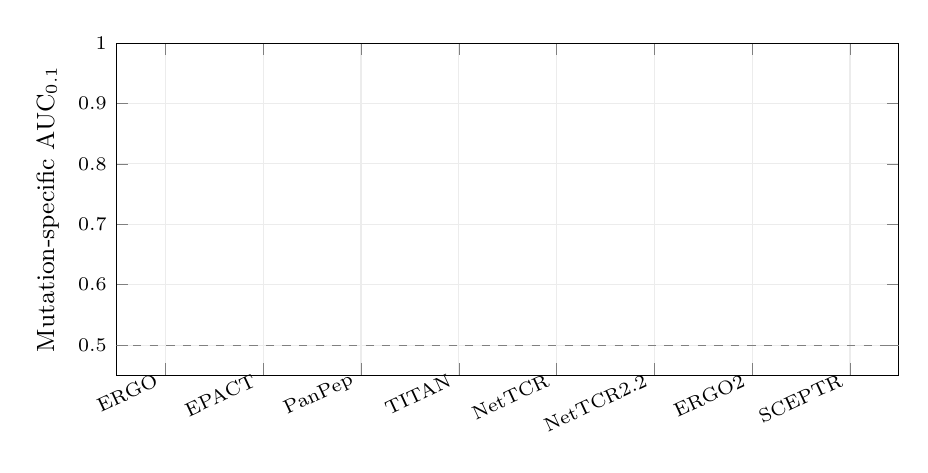
\begin{tikzpicture}
\begin{axis}[
    width=0.95\linewidth,
    height=5.8cm,
    ylabel={Mutation-specific AUC$_{0.1}$},
    xmin=0.5,
    xmax=8.5,
    ymin=0.45,
    ymax=1.0,
    xtick={1,2,3,4,5,6,7,8},
    xticklabels={
        ERGO,
        EPACT,
        PanPep,
        TITAN,
        NetTCR,
        NetTCR2.2,
        ERGO2,
        SCEPTR
    },
    xticklabel style={
        rotate=25,
        anchor=east,
        font=\scriptsize
    },
    ytick={0.5,0.6,0.7,0.8,0.9,1.0},
    tick label style={font=\scriptsize},
    label style={font=\small},
    grid=major,
    grid style={draw=gray!15},
    boxplot/draw direction=y
]

% Random-reference line
\draw[dashed,gray]
    (axis cs:0.5,0.5) --
    (axis cs:8.5,0.5);

% Data: analysis/exp3.py -> mutation_specific_auc.csv (via make_figure_data.py).
% Whiskers are min/max; quartiles use linear interpolation. Row order = draw_position.

% Row order in fig4_mutation_auc_boxstats.csv: ERGO, EPACT, PanPep, TITAN, NetTCR, NetTCR2.2, ERGO2, SCEPTR

\boxfromtable{0}{1}  % ERGO
\boxfromtable{1}{2}  % EPACT
\boxfromtable{2}{3}  % PanPep
\boxfromtable{3}{4}  % TITAN
\boxfromtable{4}{5}  % NetTCR
\boxfromtable{5}{6}  % NetTCR2.2
\boxfromtable{6}{7}  % ERGO2
\boxfromtable{7}{8}  % SCEPTR

\end{axis}
\end{tikzpicture}%
%

\caption{
\textbf{Mutation-specific prediction performance.}
Distribution of mutation-specific AUC$_{0.1}$ values across the
\valNeligible\ variants containing both experimentally positive and negative
TCR interactions. Prediction performance varies substantially across
individual substitutions for all eight models. The dashed line indicates
the random-reference level of 0.5.
}
\label{fig:mutation_auc_distribution}

\end{figure}

% ============================================================
% Figure 4: Position-level mean AUC heatmap
% ============================================================

\begin{figure}[!htbp]
\centering

% fig5: generated from templates/fig5.tex.in by stages/stage7_figures.py
\input{../results/figures/fig5.tex}%

\caption{
\textbf{Position-specific prediction performance.}
Mean mutation-specific AUC$_{0.1}$ for each model at each peptide
position. Each value averages the AUC$_{0.1}$ values of all
AUC-eligible substitutions at that position. Black outlines identify
the highest-performing model at each position. P1 is omitted because
none of its substitutions contained both experimental classes.
}
\label{fig:position_auc_heatmap}

\end{figure}

% ============================================================
% Figure 5: R5 vs non-R5 prediction performance
% ============================================================

\begin{figure}[!htbp]
\centering

% fig6: generated from templates/fig6.tex.in by stages/stage7_figures.py
% GENERATED - edit templates/fig6.tex.in and re-run stage 7, not this file.
% GENERATED from templates/fig6.tex.in by stages/stage7_figures.py into results/figures/fig6.tex
% A DATA placeholder is replaced with the source table's filename; pgfplots finds it via
% the table search path set by the including document. Edit this file to change the figure.
\begin{tikzpicture}
\begin{axis}[
    width=0.95\linewidth,
    height=5.8cm,
    ybar,
    bar width=7pt,
    ymin=0.45,
    ymax=0.70,
    ylabel={Mean AUC$_{0.1}$},
    xlabel={Model},
    symbolic x coords={
        ERGO,
        EPACT,
        PanPep,
        TITAN,
        NetTCR,
        NetTCR2.2,
        ERGO2,
        SCEPTR
    },
    xtick=data,
    xticklabel style={
        rotate=25,
        anchor=east,
        font=\scriptsize
    },
    ytick={0.5,0.55,0.60,0.65,0.70},
    tick label style={font=\scriptsize},
    label style={font=\small},
    legend style={
        at={(0.5,1.04)},
        anchor=south,
        legend columns=2,
        font=\scriptsize,
        draw=none
    },
    grid=major,
    grid style={draw=gray!15}
]

% Random-reference line
\draw[dashed,gray]
    (axis cs:ERGO,0.5) --
    (axis cs:SCEPTR,0.5);

% Data: analysis/exp3.py -> r5_vs_nonr5_auc_summary.csv (via make_figure_data.py)
% R5 mutations
\addplot table[x=model,y=r5,col sep=comma]
    {fig6_source.csv};

% non-R5 mutations
\addplot table[x=model,y=non_r5,col sep=comma]
    {fig6_source.csv};

\legend{R5, non-R5}

\end{axis}
\end{tikzpicture}%
%

\caption{
\textbf{Prediction performance for R5 and non-R5 mutations.}
Mean AUC$_{0.1}$ was calculated across the \valNrfive\ R5 substitutions
and the \valNnonrfive\ AUC-eligible non-R5 substitutions, respectively.
R5 mutations were more difficult to predict for all eight models.
The dashed line indicates the random-reference level of 0.5.
}
\label{fig:r5_model_performance}

\end{figure}


\subsection{Prediction difficulty increases with experimentally observed mutation severity}

The preceding analyses showed that model performance varies substantially
across individual mutations and peptide positions. We next examined whether
this variation follows a systematic pattern that can help characterize the
failure modes of current TCR--epitope prediction models. Specifically, we
asked whether mutations that produce larger experimentally observed changes
in TCR recognition are also more difficult for the tested models to predict.

To characterize mutation severity, we used two complementary experimental
measures. The first captures the magnitude of the mutation effect and is
defined as the mean decrease in log$_2$ fold-change relative to the reference
YLQPRTFLL peptide across the tested TCRs. The second captures the breadth of
the effect and is defined as the binder-loss fraction, i.e., the proportion
of tested TCRs that no longer satisfy the experimentally defined binding
criterion for the mutant peptide.

For each AUC-eligible mutation, we compared these measures with the mean
mutation-specific AUC$_{0.1}$ across the eight evaluated models. As shown in
Fig.~\ref{fig:severity_vs_prediction}a, prediction performance decreased as
the experimentally measured magnitude of recognition loss increased.
Experimental disruption was negatively correlated with cross-model
AUC$_{0.1}$ (Spearman $\rho=-\valRhoDisruption$, $p=\valPDisruption$).

A similar and even stronger pattern was observed for the binder-loss fraction
(Fig.~\ref{fig:severity_vs_prediction}b). Mutations that caused loss of
binding across a larger fraction of TCRs were associated with lower
prediction performance (Spearman $\rho=-\valRhoBinderLoss$,
$p=\valPBinderLoss$).

These results characterize an important failure mode of the evaluated
models. Prediction difficulty is not distributed uniformly across antigen
mutations; rather, the models perform worst on mutations that produce the
largest or broadest experimentally observed changes in TCR recognition.
This extends the position-level findings by showing that the difficulty of
R5 substitutions reflects a broader relationship between mutation severity
and prediction performance across the mutation landscape.

% ============================================================
% Figure: Experimental mutation severity vs prediction difficulty
% ============================================================

\begin{figure*}[!t]
\centering

% ============================================================
% Panel A: Continuous experimental disruption
% ============================================================

\begin{subfigure}[t]{0.48\textwidth}
\centering

% fig7a: generated from templates/fig7a.tex.in by stages/stage7_figures.py
% GENERATED - edit templates/fig7a.tex.in and re-run stage 7, not this file.
% GENERATED from templates/fig7a.tex.in by stages/stage7_figures.py into results/figures/fig7a.tex
% A DATA placeholder is replaced with the source table's filename; pgfplots finds it via
% the table search path set by the including document. Edit this file to change the figure.
\begin{tikzpicture}
\begin{axis}[
    width=\linewidth,
    height=6.0cm,
    xlabel={Experimental disruption},
    ylabel={Mean AUC$_{0.1}$ across models},
    xmin=1.2,
    xmax=5.0,
    ymin=0.47,
    ymax=0.82,
    tick label style={font=\scriptsize},
    label style={font=\small},
    grid=major,
    grid style={draw=gray!15}
]

% Random-reference level
\draw[dashed,gray]
    (axis cs:1.2,0.5) --
    (axis cs:5.0,0.5);

% One point per AUC-eligible mutation
\addplot[
    only marks,
    mark=*,
    mark size=1.8pt
]
table[
    x=Experimental_Disruption,
    y=Mean_AUC01,
    col sep=comma
]{fig7_source.csv};

% Optional linear trend line
\addplot[
    no marks,
    thick
]
table[
    x=Experimental_Disruption,
    y={create col/linear regression={y=Mean_AUC01}},
    col sep=comma
]
{fig7_source.csv};

\end{axis}
\end{tikzpicture}%
%

\caption{
Relationship between continuous experimental mutation disruption and
prediction performance. Experimental disruption is defined as the negative
mean change in log$_2$ fold-change relative to the reference peptide, such
that larger values indicate stronger loss of TCR recognition. Each point
represents one AUC-eligible mutation. Prediction performance is averaged
across the eight evaluated models. Spearman $\rho=-\valRhoDisruption$
($p=\valPDisruption$).
}
\label{fig:severity_disruption}
\end{subfigure}%
\hfill%
% ============================================================
% Panel B: Binder-loss fraction
% ============================================================
\begin{subfigure}[t]{0.48\textwidth}
\centering

% fig7b: generated from templates/fig7b.tex.in by stages/stage7_figures.py
\input{../results/figures/fig7b.tex}%

\caption{
Relationship between experimentally observed binder loss and prediction
performance. Binder-loss fraction is the proportion of tested TCRs that
lose experimentally defined binding for a given mutation. Mutations causing
greater loss of recognition are substantially more difficult for current
prediction models. Spearman $\rho=-\valRhoBinderLoss$
($p=\valPBinderLoss$).
}
\label{fig:severity_binderloss}
\end{subfigure}

\caption{
\textbf{Experimentally disruptive antigen mutations are more difficult
for current TCR--epitope prediction models.}
(a) Cross-model prediction performance decreases as the experimentally
measured reduction in TCR recognition becomes larger.
(b) An even stronger relationship is observed when mutation severity is
measured by the fraction of TCRs that lose binding. Each point represents
one of the \valNeligible\ mutations supporting AUC$_{0.1}$ evaluation, and the
y-axis shows the mean mutation-specific AUC$_{0.1}$ across the eight
evaluated models. Dashed lines indicate the random-reference value of 0.5.
}
\label{fig:severity_vs_prediction}
\end{figure*}


\section{Discussion}

This study evaluates TCR--epitope prediction from a mutation-aware perspective rather than relying only on conventional pairwise binding classification. Using the experimentally characterized YLQPRTFLL mutation landscape, we found that current models provide only modest overall discrimination across antigen variants and that prediction performance varies substantially across both individual mutations and peptide positions. No single model consistently performed best across the antigen sequence, suggesting that current approaches capture different and incomplete aspects of TCR recognition.

The position-specific analysis further showed that model difficulty reflects biologically meaningful structure in the experimental landscape. In particular, substitutions at the central R5 residue, which produced the strongest experimental loss of recognition, were also more difficult to predict than mutations at other positions. More generally, prediction performance decreased as mutations produced stronger or broader experimentally observed disruption of TCR recognition. This result is important because it indicates that model errors are not uniformly distributed across mutation space. Instead, current predictors tend to perform worst on mutations that have the largest biological consequences for TCR recognition.

These findings complement recent benchmarking studies showing limited generalization of TCR--epitope prediction models to unseen or underrepresented antigen settings. Conventional benchmarks primarily ask whether a model can distinguish positive from negative TCR--epitope pairs. Our results suggest that even when models provide useful discrimination at the interaction level, this does not necessarily imply that they can accurately predict the consequences of antigen sequence variation. Mutation-aware evaluation therefore exposes limitations that may remain hidden in aggregate benchmark performance.

The results also have implications for future model development. Improved TCR--epitope predictors may need to capture not only sequence compatibility between a TCR and peptide, but also the structural and biochemical consequences of localized antigen perturbations. The substantial variation in model performance across positions suggests that current sequence representations do not fully encode positional constraints governing TCR recognition. Training and evaluation datasets containing systematic mutational perturbations may therefore be valuable for developing models that generalize more reliably to antigenic variation.

Several limitations should be noted. The benchmark is based on a single HLA-A*02:01-restricted SARS-CoV-2 epitope and 21 TCRs, and the observed positional patterns may not generalize directly to other epitopes, HLA alleles, or TCR repertoires. In addition, although the systematic mutation panel provides dense coverage of local antigen sequence space, it evaluates only single-amino-acid substitutions. Future studies should extend mutation-aware benchmarking to additional antigens, HLA contexts, larger TCR repertoires, and combinations of mutations.

Overall, this work shows that mutation-aware evaluation provides information that is complementary to conventional TCR--epitope benchmarks. By linking prediction performance directly to experimentally measured antigen perturbations, the framework helps identify not only how well current models perform, but also which types of biologically consequential mutations remain difficult to predict.

\section{Conclusion}

We developed a mutation-aware benchmark for evaluating whether current
TCR--epitope prediction models reproduce experimentally observed effects of
single-amino-acid antigen variation. Across eight representative models,
overall discrimination was modest, prediction performance varied substantially
across mutations and peptide positions, and no single model performed best
throughout the antigen sequence. Mutations at the experimentally restrictive
R5 position were particularly difficult to predict, and more generally,
prediction performance declined as mutations produced stronger or broader
losses of TCR recognition.

These results show that conventional TCR--epitope binding performance does
not fully characterize a model's ability to predict the consequences of
antigen sequence variation. Mutation-aware benchmarking provides a
complementary evaluation perspective that can help identify biologically
important failure modes and guide the development of models that generalize
more reliably to antigenic variation.
\bibliographystyle{plain}
\bibliography{bio,references} 

\end{document}